\documentclass[conference]{IEEEtran}
% Draft 1, 30 Oct 2026. Every measured number is a macro from generated/metrics.tex (make_metrics.py), traced in
% generated/metrics_sources.md; design constants of the controller (deadline, frame rate, budgets, step sizes) are
% the defaults of validation/hardware/adaptive2.py and are written out.
\usepackage{amsmath,amssymb}
\usepackage{booktabs}
\usepackage{graphicx}
\usepackage{tikz}
\usetikzlibrary{positioning,arrows.meta}
\usepackage{cite}
\usepackage{url}
\usepackage[hidelinks]{hyperref}
\input{generated/metrics.tex}

\begin{document}
\title{Pricing the Camera Drone's Power in Streaming Perception:\\A Measured Study of Three-Tier Detection Offloading}
\author{\IEEEauthorblockN{Utkarsh Sengar}
\IEEEauthorblockA{Department of Computer Science \& Engineering, Indian Institute of Technology Dharwad, India\\
cs23bt026@iitdh.ac.in}}
\maketitle

\begin{abstract}
A camera drone that detects objects in its video can run the detector on its own small computer, on an edge drone,
or on a ground GPU, and a scheduler must choose one for every frame. We study this choice on real hardware: a fanless
Raspberry Pi~5 camera drone, a Jetson Orin Nano edge drone and a ground GPU, over Wi-Fi and a batman-adv mesh, scored
with streaming AP on VisDrone video. Our controller values each frame by the accuracy its result will still have when
it is shown, using the measured decay of stale detections after motion forecasting, and prices the camera drone's
measured power and the freshness of its results with online dual variables. Pricing power does not cost accuracy: on
Wi-Fi it raised streaming AP by \EnGain{} ($\pm$\EnGainCi{}, \EnPairs{} pairs) and \EnRepGain{} in a replication; on
the mesh removing the prices left accuracy almost unchanged but cost \MeshNoPriceW{}~W and \MeshNoPriceC{}~$^\circ$C
and throttled the board \MeshNoPriceThrottle{}\,\% of the time. The objective must use the decay curve of the forecaster
that runs: built on the curve without forecasting, the same controller loses \MainNoFc{}. Where the decision should be
made depends on the mesh topology. Against an AccuMO-style 30-frame model-predictive planner, re-implemented in a
validated trace replay, the greedy priced choice is equal within the replay's error, at a fraction of the computation.
\end{abstract}

\section{Introduction}
Object detection on a drone has three places to run: the drone's own computer, an edge drone that flies with it, and a
ground station. The drone's computer is slow, heats up and has a battery; the radio links to the others fade, congest
and drop. Offloading and per-frame adaptation are well studied for phones and cameras~\cite{Ra_2011,Chen_2015,Zhang_2021},
streaming perception defines how to score a detector whose results arrive late~\cite{Li_2020,Yang_2022}, and multi-hop
UAV offloading has been built on testbeds~\cite{Coletta_2023}. What has not been measured is how the camera drone's
power and heat interact with streaming accuracy when a scheduler can use all three tiers.

We built and measured such a system and report four findings, each from paired hardware campaigns unless marked:
\begin{itemize}
\item \emph{Pricing the camera drone's power holds or raises streaming accuracy.} A dual-ascent price on the measured
board power removes low-value onboard inference; on Wi-Fi this raised streaming AP (\EnGain{} and \EnRepGain{} in two
campaigns of \EnPairs{} pairs; \EnVdGain{} and \EnRepVdGain{} with the standard metric and VisDrone-trained detections,
Holm $p=\EnVdHolm{}$ and \EnRepVdHolm{}), and on the mesh it kept accuracy while removing throttling
(Section~\ref{sec:energy}).
\item \emph{The objective must match the forecaster.} Valuing a result by the decay curve measured \emph{after} motion
forecasting beats the curve without forecasting and a flat curve (Section~\ref{sec:decay}).
\item \emph{Where to decide depends on the topology.} With a direct ground link the camera drone should choose among all
tiers; when the ground is reachable only through the edge drone, letting the edge drone decide is better
(Section~\ref{sec:topology}).
\item \emph{A greedy priced choice does as well as planning (trace replay).} An AccuMO-style planner~\cite{Kong_2023}
ties our controller within the replay's known error (Section~\ref{sec:planner}).
\end{itemize}
We also report negative results: a heat price adds nothing beyond the energy price, and pricing the edge drone's energy
saves little because its power is dominated by idle draw (Section~\ref{sec:negative}). Finally, we measure a first
two-camera hardware swarm and a calibrated swarm simulation (Section~\ref{sec:swarm}).

\section{Related Work}
\textbf{Offloading and adaptation.} Odessa~\cite{Ra_2011} adapts offloading and parallelism for interactive perception,
Glimpse~\cite{Chen_2015} tracks objects on the device to hide offloading delay, and Elf~\cite{Zhang_2021} splits frames
across servers; configuration and bandwidth adaptation for video analytics is studied in Chameleon~\cite{Jiang_2018},
AWStream~\cite{Zhang_2018} and~\cite{Zhang_2022,Du_2020}.
Detection-specific offloading triggers use confidence (OffloaD~\cite{Gomez_2024}) or an estimated offloading
reward~\cite{Qiu_2024}; we re-implement both as baselines.
\textbf{Streaming perception.} Li et al.~\cite{Li_2020} score a detector by the accuracy of the result available at
each frame; StreamYOLO~\cite{Yang_2022} and Chanakya~\cite{Ghosh_2023} improve or adapt the detector, and StreamFlow
applies optical-flow forecasting to UAV video~\cite{Wang_2025}. We score a distributed offloading system with it.
\textbf{Accuracy-aware scheduling.} AccuMO~\cite{Kong_2023} predicts how accuracy decays between offloads and plans over
a horizon; AoPI~\cite{Li_2024} optimises freshness and accuracy of video analytics at the edge. Neither prices energy
or heat. LEAF~\cite{Wang_2023} trades energy against accuracy with a fixed weight; energy-aware DNN offloading and offloading
under energy or latency budgets are studied in~\cite{Xu_2021,Jiang_2023,Younis_2024}, and quality-aware offloading for
cooperative perception in~\cite{Zaki_2024}; Phoenix~\cite{Jeon_2026} manages on-device inference under thermal limits.
\textbf{UAV offloading.} A$^2$-UAV~\cite{Coletta_2023} optimises DNN offloading over a multi-hop UAV testbed; Qu et al.~\cite{Qu_2024} orchestrate
video analytics across a drone network edge; multi-UAV edge computing is mostly studied analytically~\cite{Sun_2024,Hao_2024}.
\textbf{Split computing.} Splitting the detector between drone and server~\cite{kang2017neurosurgeon,matsubara2022survey}
and learned feature compression~\cite{Matsubara_2022,Furutanpey_2024} are alternatives to sending the image; on our
hardware the image is the better payload (companion study), so the controller sends JPEG frames.

\section{System}\label{sec:system}
\begin{figure}[t]
\centering
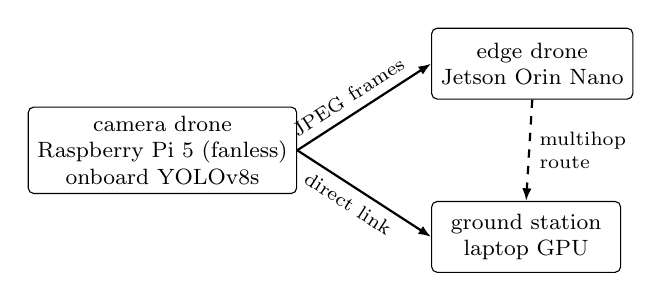
\begin{tikzpicture}[node distance=6mm and 17mm, font=\footnotesize,
  box/.style={draw, rounded corners=2pt, align=center, minimum width=24mm, minimum height=9mm},
  link/.style={-{Latex[length=1.6mm]}, thick}]
\node[box] (cam) {camera drone\\Raspberry Pi 5 (fanless)\\onboard YOLOv8s};
\node[box, right=of cam, yshift=11mm] (edge) {edge drone\\Jetson Orin Nano};
\node[box, right=of cam, yshift=-11mm] (gnd) {ground station\\laptop GPU};
\draw[link] (cam.east) -- node[above, sloped, pos=0.45, font=\scriptsize] {JPEG frames} (edge.west);
\draw[link] (cam.east) -- node[below, sloped, pos=0.45, font=\scriptsize] {direct link} (gnd.west);
\draw[link, dashed] (edge.south) -- node[right, font=\scriptsize, align=left] {multihop\\route} (gnd.north);
\end{tikzpicture}
\caption{Testbed. Every frame is detected onboard or sent as a JPEG to the edge drone or the ground station, over Wi-Fi or
a batman-adv mesh; in the multihop topology the direct link is blocked and the route crosses the edge drone. Results
return to the camera drone.}
\label{fig:testbed}
\end{figure}
\textbf{Tiers and links} (Fig.~\ref{fig:testbed}). The camera drone is a Raspberry Pi~5 without a fan (YOLOv8s: \PiFullMs~ms per frame once it
throttles); the edge drone is a Jetson Orin Nano (\JetsonFullMs~ms, FP16); the ground station is a laptop GPU. The Pi
reaches the Jetson and the ground over Wi-Fi or over an ad-hoc batman-adv mesh, on which the route to the ground can be
forced through the Jetson (multihop). Link faults (rate limits, loss, blackouts) are applied per phase with
\texttt{netem} on the camera drone.
\textbf{Workload and metric.} The camera streams the VisDrone2019-VID validation clips~\cite{zhu2022visdrone} at
30~frames/s. Detectors are YOLOv8~\cite{jocher2023yolo} models fine-tuned on VisDrone (onboard: YOLOv8s at 320 or
640~px; servers: YOLOv8s at 320--640~px and YOLOv8m at 640~px, JPEG quality 90 or 50). Accuracy is streaming AP (sAP): at every frame
the newest result that has arrived is scored against that frame's labels, with a camera-motion-aligned forecaster that
moves stale boxes forward, running live on the Pi.

\section{Controller}\label{sec:controller}
Every camera tick each idle server $s$ proposes its best setting $v$, and the frame goes to the server with the
largest value. The value of a result is the accuracy it provides while it is held:
\begin{equation}
\begin{split}
V(s,v) = {} & \frac{A_v}{A_{\mathrm{ref}}}\,H(L,T)\,p_{\mathrm{late}} - \mu\,E_{\mathrm{cam}}(s,v)\\
 & + \lambda_F\,p_{\mathrm{on}}\,\mathbf{1}[\mathrm{AoI}+L\ge D],
\end{split}
\end{equation}
where $A_v$ is the measured accuracy of setting $v$, $L$ the expected latency (encode, transfer at the live goodput
estimate, server time, round trip), $T$ how long the result will be held, $H(L,T)$ the mean of the measured decay
$\rho(\cdot)$ of streaming accuracy over the holding window, $p_{\mathrm{on}}$ and $p_{\mathrm{late}}$ the probabilities
of arriving within the 300~ms deadline $D$ and a 1~s late window under Gaussian goodput uncertainty, and $E_{\mathrm{cam}}$
the camera drone's measured energy for the frame (onboard inference, or encoding and radio). The decay $\rho$ is
measured on the training clips with the forecaster that runs (Fig.~\ref{fig:decay}).

\begin{figure}[t]
\centering
\includegraphics[width=\columnwidth]{figures/decay.pdf}
\caption{Streaming accuracy kept by a result shown late (VisDrone-VID train clips): without correction, with object
velocity forecasting, and with camera-aligned forecasting. The controller's objective uses the curve of the forecaster
that runs.}
\label{fig:decay}
\end{figure} The energy price follows the measured board power
$\bar P$: $\mu \leftarrow \max(0, \mu + 0.1(\bar P - 2.8\,\mathrm{W}))$ once per second, with a thermal guard and no
price on onboard inference while no link can deliver. The freshness price follows the share $\hat F$ of the last 5~s
with a result younger than $D$: $\lambda_F \leftarrow \max(0, \lambda_F + 2(0.95 - \hat F))$. The heat-priced variant
replaces $\mu$ by $\mu + \lambda_T$, with $\lambda_T$ driven by a measured thermal model's 60~s prediction; the edge-priced
variant subtracts $\mu_e E_{\mathrm{edge}}$ for the Jetson's measured energy.

\section{Method}\label{sec:method}
Strategies are compared in paired campaigns: every repetition runs all strategies on the same scenario, in shuffled
order, with the same scripted link faults, following common advice on benchmarking with repetitions~\cite{Kalibera_2013}. Differences are reported as paired means with Student-$t$ 95\,\%
intervals; $p$-values are exact sign-permutation tests, Holm-corrected over the comparisons of a campaign where
stated. The board's power and temperature are measured (PMIC rails, 5~Hz); the Jetson's power is logged from its
INA3221 sensor. Comparisons that cannot be run on hardware (a published planner, hindsight oracles) use a trace replay
rebuilt from the recorded runs; against the 240 runs of the main campaign it reproduces per-policy streaming AP with
$r=\ReplaySapR{}$, but it favours policies that run less onboard by about \ReplayLeafBias{}~sAP.

\section{Results}
\begin{table*}[t]
\centering
\caption{Headline paired comparisons (streaming AP with forecaster; difference $\pm$ 95\,\% interval; positive = the
first strategy is better). Camera: measured change of the camera drone's power and temperature.}
\label{tab:results}
\small
\begin{tabular}{@{}llrrl@{}}
\toprule
Comparison & Where & $\Delta$ sAP & Pairs & Camera \\ \midrule
v4 $-$ v3+fc (no price) & Wi-Fi & \EnGain{}$\pm$\EnGainCi{} & \EnPairs{} & \\
v4 $-$ v3+fc, replication & Wi-Fi & \EnRepGain{}$\pm$\EnRepCi{} & 20 & \\
v4.1 $-$ no prices & mesh & \MeshNoPriceSap{}$\pm$\MeshNoPriceSapCi{} & \MeshPairs{} & $-$\MeshNoPriceW{}~W, $-$\MeshNoPriceC{}~$^\circ$C \\
heat price $-$ v4.1 & mesh & \HeatSap{}$\pm$\HeatSapCi{} & \MeshPairs{} & +\HeatW{}~W, +\HeatC{}~$^\circ$C \\
v3+fc $-$ v2 (rate) & Wi-Fi & \FcGain{}$\pm$\FcGainCi{} & \FcPairs{} & \\
v5, decay without fc $-$ v5 & Wi-Fi & \MainNoFc{}$\pm$\MainNoFcCi{} & 20 & \\
v5, flat decay $-$ v5 & Wi-Fi & \MainFlat{}$\pm$\MainFlatCi{} & 20 & \\
camera decides $-$ chain, direct & mesh & \TopoDirectDiff{}$\pm$\TopoDirectDiffCi{} & \TopoDirectPairs{} & \\
camera decides $-$ chain, multihop & mesh & \TopoMultiDiff{}$\pm$\TopoMultiDiffCi{} & \TopoMultiPairs{} & \\
AccuMO-style $-$ v4.1, random faults & replay & \MpcRandom{}$\pm$\MpcRandomCi{} & \MpcRandomN{}$^\dagger$ & \\
\bottomrule
\multicolumn{5}{@{}l}{$^\dagger$seeds of the trace replay, not hardware pairs.}
\end{tabular}
\end{table*}

\subsection{Pricing power holds or raises accuracy}\label{sec:energy}
On Wi-Fi, the energy-priced controller (v4) against the same controller without prices (v3 with forecasting) gained
\EnGain{}$\pm$\EnGainCi{}~sAP, ahead in \EnWins{} of \EnPairs{} pairs; a second campaign gave
\EnRepGain{}$\pm$\EnRepCi{} (ahead in \EnRepWins{} of 20). Re-scored with the standard metric and detections of the
VisDrone-trained detector, the gains are \EnVdGain{} and \EnRepVdGain{} (Holm $p=\EnVdHolm{}$, \EnRepVdHolm{}). On the
mesh (\MeshPairs{} pairs over three scenarios), removing the prices from v4.1 left streaming AP almost unchanged
(v4.1 ahead by \MeshNoPriceSap{}, $p=\MeshNoPriceP{}$) but cost \MeshNoPriceW{}~W and \MeshNoPriceC{}~$^\circ$C on the
camera drone ($p=\MeshNoPriceWp{}$, every pair), and the board throttled \MeshNoPriceThrottle{}\,\% of the time against
\MeshVThrottle{}\,\% with prices. Over 24-minute mesh missions v4.1 held \MeshLongSap{}~sAP with the board throttled
\MeshLongThrottle{}\,\% of the time (\MeshLongN{} runs). The mechanism, less low-value onboard inference and therefore
less heat and CPU contention, is consistent with these measurements but was not isolated by an ablation.

\textbf{The whole system.} These gains are for the camera drone. Counting the power of every board, including the edge
drone that carries the Jetson, fixed offloading of every frame to the ground is the most accuracy-per-watt efficient
strategy: \SysEffFixed{} sAP per watt against \SysEffMin--\SysEffMax{} for the priced controllers (a factor of
\SysEffRatioMin--\SysEffRatioMax), because it needs no edge drone. It holds a fresh result only \SysFixedAvail\,\% of
the time (the priced controllers at least \SysVAvailMin\,\%) and fails when its link fails, so the edge drone's case is
robustness, not energy.

\subsection{The objective must match the forecaster}\label{sec:decay}
With the decay curve after forecasting, the streaming objective beat the rate objective of v2 by
\FcGain{}$\pm$\FcGainCi{}~sAP (\FcPairs{} pairs). In the 240-run main campaign the priced controller (v5) with the curve
measured without forecasting lost \MainNoFc{}$\pm$\MainNoFcCi{}, and with a flat curve \MainFlat{}$\pm$\MainFlatCi{}; generic
linear and exponential decays on the deadline's time scale tied (\MainLin{}, \MainExp{}). What matters is a decay as
slow as the forecaster makes it, not the exact measured shape.

\subsection{Where the decision belongs}\label{sec:topology}
On the mesh with a direct camera-to-ground link, the camera deciding among all tiers (v4.1) reached \TopoDirectV{}~sAP
against \TopoDirectH{} for a hierarchical chain in which the edge drone decides (\TopoDirectPairs{} pairs,
$p=\TopoDirectP{}$). With the direct link blocked so that every packet crosses the edge drone, the order reversed:
\TopoMultiH{} for the chain against \TopoMultiV{} for v4.1 (3 pairs).

\subsection{Published schedulers and a planner}\label{sec:planner}
In the main campaign the re-implemented literature schedulers (confidence trigger~\cite{Gomez_2024}, offloading
reward~\cite{Qiu_2024}, freshness threshold, shortest queue) differed from the priced controller (v5) by \MainLitMin{}
to \MainLitMax{}~sAP (20 pairs each), and a LEAF-style fixed weight~\cite{Wang_2023} tied it (\MainLeaf{}). We re-implemented an
AccuMO-style planner in the trace replay: one setting per server for the next 30 frames (252 plans), the
content-conditioned decay, the plan maximising the accuracy of the result on screen. Against the priced controller it
was \MpcMission{}$\pm$\MpcMissionCi{} on the mission (\MpcMissionN{} seeds), \MpcRandom{}$\pm$\MpcRandomCi{} on random
link faults and \MpcLong{}$\pm$\MpcLongCi{} over 24-minute missions; the LEAF-style weight was ahead by as much
(\LeafMission{}, \LeafRandom{}, \LeafLong{}). On fresh seeds with a corrected onboard power model the random-link
difference was \MpcHeldRandom{}$\pm$\MpcHeldRandomCi{}. All of these are within the replay's known bias towards light
onboard use (\ReplayLeafBias{}), so the supported claim is that the greedy priced choice does as well as a 30-frame
planner here; the planner takes \MpcMs{}~ms per frame on a laptop CPU, and its hardware comparison is future work.

\textbf{Distance from the best schedule (trace replay).} Knowing the exact goodput of every next transfer in advance
changes v4.1's streaming AP by at most \ClairMax{} (inside the interval in every scenario), so a better link predictor
would not help under the emulated faults. Against a hindsight oracle that picks, per network phase, the best of v4.1
and 17 fixed settings, v4.1 reaches \OracleShareMin--\OracleShareMax\,\% of the oracle's accuracy with 20~s phases and
\OracleShareRandom\,\% when the faults change every 4~s.

\textbf{Calibration (trace replay).} Over \CalFrames{} offloaded frames, v4.1 predicted on average a \CalPred\,\%
chance of meeting the deadline and \CalObs\,\% met it (expected calibration error \CalEce{}); no probability bin was
over-confident, so the controller is cautious rather than optimistic.

\subsection{Several camera drones}\label{sec:swarm}
With two real camera drones (the Pi and the Jetson as cameras) sharing the ground GPU, sharing cost the Pi
\DuoShareLossMin--\DuoShareLossMax\,\% of its streaming AP, and adaptive control on both cameras beat fixed offloading
by \DuoAdaptGain{}$\pm$\DuoAdaptCi{} (\DuoAdaptWins{} of \DuoPairs{} pairs). A ground-side admission coordinator
rarely acted with two cameras (\DuoCoordGain{}$\pm$\DuoCoordCi{}). In a swarm simulation calibrated with the measured
boards and links, 20 Pi camera drones on one Wi-Fi access point each delivered \SwarmTwentyAlone{} detections/s when
every drone adapted alone and \SwarmTwentyCoord{} with the coordinator; larger hardware swarms are future work.

\subsection{Negative results}\label{sec:negative}
A predictive heat price added nothing beyond the energy price: same accuracy (\HeatSap{}) at \HeatW{}~W and
\HeatC{}~$^\circ$C more on the camera drone ($p=\HeatP{}$). Pricing the Jetson's energy at a 0.5~W budget cost
\JetHalfSap{}~sAP, and at 1.2~W \JetTwelveSap{} ($p=\JetTwelveP{}$), for little saving, because the edge drone's power is
dominated by its idle draw.

\section{Limitations}
The boards were on a table, one hop apart, with recorded video replayed; the mesh runs batman-adv as is, one of several
routing protocols compared for UAV meshes~\cite{Diniz_2025}, and its own effect was not characterised; there was one
camera drone on the mesh; most
mesh cells have 3 repetitions; the trace replay favours low-onboard policies by about \ReplayLeafBias{}~sAP, so the
planner comparison is provisional; the energy mechanism is not isolated by an ablation.

\section{Conclusion}
On a real three-tier drone system, a greedy scheduler that values each frame by the accuracy its result will still
have, and prices the camera drone's measured power and the freshness of its results, keeps or raises streaming
accuracy while removing thermal throttling. Its objective must use the decay curve of the forecaster in use, and the
best place to decide depends on the mesh topology.

\bibliographystyle{IEEEtran}
\bibliography{references}
\end{document}
